\SECTION{Evaluation}\label{sec:evaluation}
In this section, we evaluate the runtime overhead and real-time
performance of Linux-RTXG.
The runtime overhead is classified into interrupt interception,
independent synchronization, and priority-driven scheduling in Linux.
We demonstrate that the overhead of our LKM-based real-time scheduler
for GPU applications is acceptable.
The real-time performance is verified in terms of QoS management and
prioritization using both synthetic workload and real-world
applications on top of three different device drivers -- NVIDIA,
Nouveau, and Gdev.
We demonstrate that multiple GPU applications co-scheduled by our
LKM-based real-time scheduler are successfully prioritized and
maintained at the desired frame rate even in the presence of high CPU
load.

Experiments are limited to GPU scheduling performance given that CPU
scheduling performance has already been demonstrated in previous
work~\cite{kato2009loadable}.
Considering the results of this work and those from the previous work,
it is clarified that both emerging GPU applications and traditional CPU
applications can be scheduled according to priorities and resource
reserves using LKMs, without modifying the Linux kernel and device
drivers.

\SUBSECTION{Experimental Setup}
Our experiments were conducted using the Linux kernel 3.16.0, an NVIDIA
Geforce GTX680 GPU, a 3.40 GHz Intel Core i7 2600 (eight cores including
two hyperthreadling cores), and 8 GB main memory.  
GPU application programs were written in CUDA and compiled by NVCC v6.0.1.
We used the NVIDIA 331.62 driver and Nouveau Linux-3.16.0 driver with
NVIDIA CUDA 6.0 and Gdev. 

\SUBSECTION{Interrupt Interception Overhead}
We measured the interrupt interception overhead using the Nouveau GPU
driver to quantify the overhead of interception in varied interrupt
types. 
As performance metrics, we adopted elapsed time from the beginning to
the end of the ISR.

\begin{figure*}[!t]
\begin{minipage}[t]{0.33\hsize}
\begin{center}
\raisebox{-3mm}{\includegraphics[width=62mm]{img/interrupt}}
\end{center}
\caption{\small{Interrupt interception overhead. \newline \,}}
\label{fig:irq_overhead}
\end{minipage}
\begin{minipage}[t]{0.33\hsize}
\begin{center}
\raisebox{-1mm}{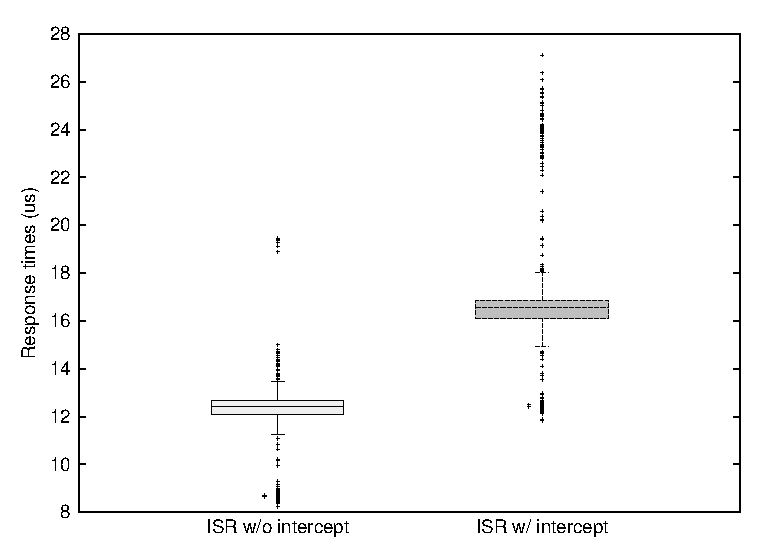
\includegraphics[width=62mm]{img/interrupt_response}}
\end{center}
\caption{\small{Impact of interrupt interception.}}
\label{fig:response}
\end{minipage}
\begin{minipage}[t]{0.33\hsize}
\begin{center}
\includegraphics[width=62mm]{img/tasklet_vs_interrupt}
\end{center}
\caption{\small{Comparison of ISR and tasklet.}}
\label{fig:bottomvstasklet}
\end{minipage}
\end{figure*}

Figure~\ref{fig:irq_overhead} shows the overhead of interrupt interception.
``Raw ISR'' represents the original implementation of ISR.
``ISR Intercept'' represents the modified ISR with the interrupt
interception mechanism, while ``ISR Intercept w/Func'' includes the
overhead of identifying the ISR and calling the scheduler thread in
addition to ``ISR Intercept''.
The average execution time in 1000 executions is presented with error
bars.

Comparing Raw ISR and ISR Intercept, the overhead of introducing the
interrupt interception mechanism was $247ns$, which is only $0.8\%$ of
Raw ISR.
Similarly, the overhead for ISR Intercept w/Func was $790ns$, which is
only $2.6\%$ of Raw ISR.
This result indicates that the interrupt interception overhead is not
significant at all for total performance.

We next compare response times of ISR with and without interrupt
interception, as shown in Figure~\ref{fig:response}.
The response time is defined by the elapsed time from the beginning of
interrupt processing to the point where the interrupt type (e.g., timer,
compute, FIFO, and GPIO) is identified. 
According to the result, the impact of interrupt interception brings
1.4x longer response times.

We also compared response times when interrupt interception is
self-contained in the ISR (top-half) and when it is expanded to the
tasklet (bottom-half).
This comparison differentiates Linux-RTXG from GPUSync in performance,
since GPUSync intercepts the $tasklet\_schedule()$ on top of the
proprietary driver, while Linux-RTXG realized ISR-based interception.
In this case, the start time of measuring the response time is set at
the function call to $do\_IRQ$.
Figure~\ref{fig:bottomvstasklet} shows the result of this comparison.
As can be seen, the tasklet-based approach requires about 5x longer
response times than the IRQ-based approach.
This occurs because the tasklet is typically called after significant
ISR processings.

\SUBSECTION{Independent Synchronization Overhead}
We next quantify the overhead of the independent synchronization
mechanism.
This mechanism must call $rtx\_gpu\_notify()$ at the time of requested
synchronization (e.g., after launching a GPU kernel).
To use this mechanism, some initialization procesure is also required.
In this measurement, the overhead is defined by the execution time of
corresponding APIs.

\begin{figure}[!t]
\begin{center}
\subfigure[Overhead of initialization]{\includegraphics[width=0.23\textwidth]{img/irq_rise_init.eps}}\subfigure[Overhead of notification]{\includegraphics[width=0.22\textwidth]{img/irq_rise_notify.eps}}
\caption{Independent synchronization overhead.}
\label{fig:irq_rise_overhead}
\end{center}
\end{figure}

Figure~\ref{fig:irq_rise_overhead} shows that the initialization
overhead could reach 5000$us$, whereas the notification overhead is no
more than a few microseconds.
The initilization procedure calls a Linux process to allocate indirect
buffers and control registers for several GPU engines.
Albeit a significant overhead, the application program is not much
affected by this procedure, since it is called only once at the
beginning.
On the other hand, the notification overhead is not a major
consideration for the application program, though it is a little
scattered due to an ioctl system call.
When NOTIFY is used to set notificaiton, the overhead was $3.5us$, while
it was reduced to $2us$ when FENCE is used.

\SUBSECTION{Scheduling Overhead}\label{sec:eval:sched_overhead}

\begin{figure}[!t]
\begin{center}
\includegraphics[width=.44\textwidth]{img/sum_task.eps}
\caption{Scheduling overhead.}
\label{fig:fp_task_overhead}
\end{center}
\end{figure}

We now evaluate the scheduling overhead posed by the presented
Linux-RTXG scheduler.
We executed three synthetic tasks -- (i) vanilla, (ii) mutex, and (iii)
rtx -- to measure the overhead. 
These tasks are based on the microbenchmark program provided by the Gdev
project, which tests a GPU loop function.
%details
We modified this program to generate multiple GPU tasks by the $fork()$
system call.
Each task releases a job ten times periodically, each of which includes
the data transfer between the CPU and the GPU, followed by GPU kernel
execution.
The rtx task was scheduled by Linux-RTXG.
The mutex task was limited to a single GPU kernel by using explicit
mutual exclusion control similar to the rtx task.
The vanilla task was not changed from the original microbenchmark
program.
The CPU scheduling policy was set to $SCHED\_FIFO$, while the GPU
scheduling policy is also based on fixed priorities with GPU resource
reservation, called the BAND scheduling policy~\cite{kato:gdev}.
The independent synchronization mechanism is employed with NOTIFY.

We measured the average time in 100 times of GPU task execution (1000 jobs).
The result is provided in Figure~\ref{fig:fp_task_overhead}.
The scheduling overhead increases in proportion as the number of tasks,
because the time consumed in queueing GPU tasks is increased. 
The maximum overhead correponds to $10\%$ of the vanilla task at eight
tasks.

\SUBSECTION{QoS Performance}
Experiments were also performed to evaluate QoS management performance.
In this evaluation, we measured the utilization of each tasks in several environments,
which indicates whether performance is affected by kernel modification.

\begin{figure*}[!t]
\begin{minipage}[t]{0.33\hsize}
\begin{center}
\subfigure[{\small FIFO with NVIDIA}]{\includegraphics[width=62mm]{img/fifo_rtx_nvidia}} 
\label{fig:fifo_rtx_nvidia} \\
\subfigure[{\small BAND with NVIDIA}]{\includegraphics[width=62mm]{img/band_rtx_nvidia}}
\label{fig:band_rtx_nvidia}
\label{fig:rtx_nvidia}
\end{center}
\end{minipage}
\begin{minipage}[t]{0.33\hsize}
\begin{center}
\subfigure[{\small FIFO with Nouveau}]{\includegraphics[width=62mm]{img/fifo_rtx}}
\label{fig:fifo_rtx} \\
\subfigure[{\small BAND with Nouveau}]{\includegraphics[width=62mm]{img/band_rtx}}
\label{fig:band_rtx}
\label{fig:rtx_nouveau}
\end{center}
\end{minipage}
\begin{minipage}[t]{0.33\hsize}
\begin{center}
\subfigure[{\small FIFO on Gdev}]{\includegraphics[width=62mm]{img/fifo_gdev}}
\label{fig:fifo_gdev} \\
\subfigure[{\small BAND on Gdev}]{\includegraphics[width=62mm]{img/band_gdev}}
\label{fig:band_gdev}
\label{fig:gdev_usage}
\end{center}
\end{minipage}
\caption{Utilization of two tasks with each scheduler. Each task had different workloads and different resource allocations (VGPU0 = 40\%, VGPU1 = 60\%).}
\label{fig:utilize}
\end{figure*}

\begin{figure}[!t]
\begin{center}
\includegraphics[width=0.4\textwidth]{img/band_rtx_fair}
\caption{Utilization of four tasks with the Linux-RTXG's BAND VGPU scheduling. Each tasks had a equal workload and a equal GPU resource allocation.}
\label{fig:band_rtx_fair}
\end{center}
\end{figure}

QoS performance use an indication of whether the task of the resource is guaranteed.
We evaluate task isolation performances with Linux-RTXG's GPU scheduler using the NVIDIA GPU driver and the Nouveau GPU driver to confirm the guaranteed resources.
First, we measured the utilization when running two GPU tasks.
Each GPU tasks had a different workload and a different GPU resource.
One GPU task was allocated VGPU0, and given the 40\% GPU resource.
This task has about 1.2 times the workload of other tasks.
The other GPU task was allocated VGPU1 and given the 60\% GPU resource.
VGPU1 task was scheduled to start approximately 5 safter the VGPU0 task.

Figure~\ref{fig:utilize}(a) shows result of FIFO scheduling policies on the NVIDIA Driver,
and the BAND scheduling policies is shown in Figure~\ref{fig:utilize}(b).

The Nouveau GPU driver results are shown in Figures~\ref{fig:utilize}(c) and (d).
The FIFO scheduling policies shown in Figure~\ref{fig:utilize}(c),
and the BAND scheduling policies shown in Figure~\ref{fig:utilize}(d).

The results shown in Figure~\ref{fig:utilize}(a) and (c) indicate that the GPU tasks are performed in accordance with the workload by fair scheduling.
The results shown in Figure~\ref{fig:utilize}(b) and \ref{fig:utilize}(d) indicate that the GPU tasks are performed in accordance with the utilization by resource reservation mechanisms.

The VGPU1 task's maximum error was approximately 3\% for the initial BAND scheduling policies' resource management using the NVIDIA GPU driver.
The VGPU0 task's maximum error was approximately 5\%.
The VGPU1 task's maximum error was approximately 2\% under the initial BAND scheduling policies' resource management using the Nouveau GPU driver.
The VGPU0 task's maximum error was approximately 2\%.
Large spikes occurred due to GPU kernel overrun.
If the GPU scheduler need to large spike is reduced, the GPU scheduler is needed for runtime approaches such as making preemptive GPU kernel.

In addition, we compare performance with prior work that is Gdev.
The Gdev scheduling results are shown in Figures~\ref{fig:utilize}(e) and (f).
Linux-RTXG is seen almost no performance degradation as compared with Gdev.
In details, the VGPU1 task's maximum error was approximately 3\% for the initial BAND scheduling policies' resource management using the Gdev scheduler.
The VGPU0 task's maximum error was approximately 5\%.
We guess that there is a large variation caused by runtime specification of the Gdev function must through the kernel module using Gdev scheduler.

We then measured utilization running four GPU tasks.
Each GPU tasks had equal workload and equal GPU resource allocation.
In addition, each GPU task was allocated to each VGPU.
Results for BAND scheduling policies are shown in Figure~\ref{fig:band_rtx_fair}.
A maximum error of these VGPUs was appropriately 9\%, it values are occurred because of the timing of budget replenishment and a synchronization latency.  

Therefore, the results show that the synchronization mechanism of the proposed Linux-RTXG can schedule tasks without sacrificing performance.

\begin{figure*}[!t]
\begin{minipage}[t]{0.33\hsize}
\begin{center}
\subfigure[{\small NULL}]{\includegraphics[width=62mm]{img/real_null_null_withoutload}}
\label{fig:real-null_null}
\subfigure[{\small FP}]{\includegraphics[width=62mm]{img/real_prio_null_withoutload}}
\label{fig:real-prio_null}
\end{center}
\end{minipage}
\begin{minipage}[t]{0.33\hsize}
\begin{center}
\subfigure[{\small BAND}]{\includegraphics[width=62mm]{img/real_prio_band_withoutload}}
\label{fig:real-prio_band}
\subfigure[{\small BAND with high CPU load}]{\includegraphics[width=62mm]{img/real_prio_band_withhighload}}
\label{fig:real-prio_band-hiload}
\end{center}
\end{minipage}
\begin{minipage}[t]{0.33\hsize}
\begin{center}
\subfigure[{\small NULL with high CPU load}]{\includegraphics[width=62mm]{img/real_null_null_withhiload}}
\label{fig:real-null_null-hiload}
\subfigure[{\small G-RM and BAND with high CPU load}]{\includegraphics[width=62mm]{img/real_prio_band_withhighload_cpu}}
\label{fig:real-prio_band_cpu-hiload}
\end{center}
\end{minipage}
\caption{Elapse times of object detection applications on various situation.}
\label{fig:elapse_time_all}
\end{figure*}

\SUBSECTION{Real-world Application}
Here, we demonstrate scheduling performance using real-world oriented application.
We employed real-world oriented application which is object detection application using the HOG features.
We run four tasks are assumed to recognize the four directions that are forward, backward, right, and left.

Algorithms and implementation of the applications are described in the previous work~\cite{hirabayashi:cpsna2013}.

We measure the elapse time of processing one frame image in six situations.
Each situation results are shown in Figure~\ref{fig:elapse_time_all}.
Each GPU tasks are allocated difference resources are given 60\%, 20\%, 10\%, and 10\% respectively.
Figure~\ref{fig:elapse_time_all}(a) is shown result of executing four tasks without scheduling.
All tasks are performed equally on its situation.
Figure~\ref{fig:elapse_time_all}(b) is shown result on executing four task runnning with a fixed-priority GPU kernel scheduling (FP).
If a scheduler only uses fixed-priority GPU kernel scheduling, tasks are almost the same as the Figure~\ref{fig:elapse_time_all}(a).
Figure~\ref{fig:elapse_time_all}(c) is addition of the BAND VGPU scheduling from the Figure~\ref{fig:elapse_time_all}(b) situation.
In this case, the tasks have been adapted the priority of each tasks for which can suppress the GPU kernel execution.
Figures~\ref{fig:elapse_time_all}(d) and (e) are shown result of the high CPU load environment.
Note that high CPU load is generated by hackbench tasks as known as an UNIX's standard stress test tool.
High CPU load tasks policy is Linux's $SCHED\_OTHER$.
If an OS has some high-CPU load tasks, GPU tasks do not work well using only GPU scheduling
because GPU tasks can not acquire the CPU to issue an API due to other tasks.
Such a high-CPU load environment to occur well in autonomouse driving car systems because the systems require a lot of applications (e.g., SLAM, Navigation, and Car control) despite limit the resources.
Linux-RTXG can provide real-time CPU scheduling and GPU scheduling.
Therefore, Linux-RTXG can solves problem due to other CPU tasks.
The result show in Figure~\ref{fig:elapse_time_all}(f).
As can be seen, applications are not affected high-CPU load task by fixed-priority CPU scheduling (G-RM:Glocbal Rate-monotonic).
These experimental results indicate that Linux-RTX making the adequate performance for real-world oriented applications.

